\documentclass[12pt]{article}
\usepackage[utf8]{inputenc}

%General Packages
\usepackage{setspace}
\usepackage{amssymb}
\usepackage{amsmath}
\usepackage{amsthm}
\usepackage{natbib}
\usepackage{xcolor}
\usepackage[shortlabels]{enumitem}
\usepackage{comment}

%Graphics package
\usepackage{graphicx}
\usepackage{caption}
\usepackage{paracol}
\usepackage{tikz}
\usepackage{subfigure}
\usepackage{tikz,pgfplots}
\usetikzlibrary{shapes,arrows}
\usetikzlibrary{quotes}
\usepgfplotslibrary{fillbetween}

\definecolor{myblue}{RGB}{101,129,177}
\definecolor{myorange}{RGB}{239,134,51}


%Page set up space
\setlength{\oddsidemargin}{0.1in}
\setlength{\evensidemargin}{0.1in}
\setlength{\topmargin}{-0.75in}
\setlength{\textwidth}{6in}
\setlength{\textheight}{9.5in}
\setlength{\parskip}{\bigskipamount}
\setlength{\parindent}{0pt}

\pgfplotsset{compat=1.18}

\newtheorem{proposition}{Proposition}

\setstretch{1.25}

\title{Your title}
\author{Your name}
\date{Date}

\begin{document}

\maketitle

\newpage

\section{Question 1}

From the given conditions, we have

\begin{paracol}{2}
    $$
        \begin{array}{l}
            \displaystyle\left. P(Y=0)=\binom{4}{3}\binom{2}{0}\middle/\binom{6}{3}\right.=\dfrac{1}{5} \\
            \displaystyle\left. P(Y=1)=\binom{4}{2}\binom{2}{1}\middle/\binom{6}{3}\right.=\dfrac{3}{5} \\
            \displaystyle\left. P(Y=2)=\binom{4}{1}\binom{2}{2}\middle/\binom{6}{3}\right.=\dfrac{1}{5} \\
        \end{array}
    $$
    Distribution of $Y$:
    \center
    \begin{tabular}{|c|c|c|c|}
        \hline
        $i$      & $0$   & $1$   & $2$   \\
        \hline
        $P(Y=i)$ & $1/5$ & $3/5$ & $1/5$ \\
        \hline
    \end{tabular}

    \switchcolumn
    \begin{tikzpicture}
        \begin{axis}[
                width=0.5\textwidth,
                height=0.4\textwidth,
                xmin=-0.5, xmax=2.5,
                ymin=0, ymax=1,
                xtick distance=1,
                minor y tick num = 3,
                title=Histogram of the distribution of $Y$,
                xlabel={$k$},
                ylabel={$P(Y=k)$},
                area style,
            ]
            \addplot+[ybar interval] plot coordinates { (-0.5,0.2) (0.5,0.6) (1.5,0.2) (3,0.2) };
        \end{axis}
    \end{tikzpicture}

\end{paracol}

\section{Question 2}

Since the PDF of $X$ is $f(x)=\left\{\begin{array}{ll}
        2x & 0<x<1 \\ 0&\text{otherwise}\end{array}\right.$, we have

$$
    \begin{array}{ll}
        \displaystyle\mathbb{E}X=\int_\mathbb{R} xf(x)dx=\int_0^1 2x^2dx=\dfrac{2}{3}     &
        \displaystyle\mathbb{E}X^2=\int_\mathbb{R} x^2f(x)dx=\int_0^1 2x^3dx=\dfrac{1}{2}   \\
        \displaystyle\mathbb{E}X^4=\int_\mathbb{R} x^4f(x)dx=\int_0^1 2x^5dx=\dfrac{1}{3} &
    \end{array}
$$

Hence

\begin{align*}
     & \mathbf{Var}(X)=\mathbb{E}(X-\mathbb{E}X)^2=\mathbb{E}X^2-(\mathbb{E}X)^2=\dfrac{1}{18}         \\
     & \mathbf{Var}(X^2)=\mathbb{E}(X^2-\mathbb{E}X^2)^2=\mathbb{E}X^4-(\mathbb{E}X^2)^2=\dfrac{1}{12} \\
\end{align*}

\section{Question 3}

\begin{enumerate}
    \item Given PDF of $Y$:

          \begin{equation*}
              f(y)=\left\{\begin{array}{ll}
                  cy & 0\leqslant y\leqslant 2 \\
                  0  & \text{otherwise}
              \end{array}\right.
          \end{equation*}

          If this is a density function, then

          $$
              \int_\mathbb{R}f(y)dy=\int_0^2 f(y)dy=\int_0^2cydy=2c=1\quad\Rightarrow\quad c=\dfrac{1}{2}
          $$

    \item $\displaystyle F(y)=\int_0^y f(y)dy=\int_0^y\dfrac{y}{2}dy=\dfrac{y^2}{4}$.
    \item $\mathbb{P}(1\leqslant Y\leqslant 2)=F(2)-F(1)=1-\dfrac{1}{4}=\dfrac{3}{4}$
    \item $\mathbb{P}(1\leqslant Y\leqslant 2)$ is the area between $x=1,x=2,f(x)$ and $y=0$ in $xOy$ axis.

              {
                  \center
                  \begin{tikzpicture}
                      \begin{axis}[
                              width=0.5\textwidth,
                              height=0.3\textwidth,
                              xmin=-0.5, xmax=2.5,
                              axis lines=center,
                              grid=major,
                              ymin=0,
                              no marks,
                          ]
                          \addplot+[smooth,orange,domain=0:2,name path=A] {x/2}; % actual curve
                          \addplot+[draw=none,name path=B] {0};     % “fictional” curve
                          \addplot+[
                              fill=yellow,
                              every path/.style={
                                      postaction={
                                              pattern=north east lines
                                          }
                                  }] fill between[of=A and B,soft clip={domain=1:1.99}]; % filling
                      \end{axis}
                  \end{tikzpicture}
              }

          The area is a trapezoid, $f(1)=\dfrac{1}{2}, f(2)=1$, hence $\mathbb{P}(1\leqslant Y\leqslant 2)=\dfrac{1}{2}(f(1)+f(2))=\dfrac{3}{4}$.

\end{enumerate}

\section{Question 4}

Denote the volumns the bottles as $X_i\sim ^{i.i.d} N(\mu,25)$, $1\leq i\leq N$, and use the estimator $\displaystyle\bar{X}=\dfrac{1}{N}\sum_{i=1}^NX_i$ for $\mu$. As we know, 
$$\bar{X}\sim N(\mu,\dfrac{25}{N})\quad\Leftrightarrow\quad \dfrac{\bar{X}-\mu}{5/\sqrt{N}}\sim N(0,1)$$
and from the table, $\Phi(-1.96)\approx0.025,\Phi(1.96)\approx 0.975$, hence
$$-1.96\leqslant\dfrac{\bar{X}-\mu}{5/\sqrt{N}}\leqslant1.96\quad\Rightarrow\quad \mu-\dfrac{9.8}{\sqrt{N}}\leqslant \bar{X}\leqslant \mu+\dfrac{9.8}{\sqrt{N}}$$
To construct a 95\%CI of width $1$, there must be $2\times \dfrac{9.8}{\sqrt{N}}\leqslant 1\ \Rightarrow\ N\geqslant \lceil (2\times 9.8)^2\rceil=385$.

\section{Question 5}

Given joint PDF:

\begin{equation*}
    f(y_1,y_2)=\left\{\begin{array}{ll}
        e^{-(y_1+y_2)} & y_1>0\text{ and }y_2>0 \\
        0  & \text{otherwise}
    \end{array}\right.
\end{equation*}

\begin{enumerate}
    \item \begin{align*}\displaystyle\mathbb{P}(Y_1<1,Y_2>5)&=\int_5^{+\infty}\int_0^1f(y_1,y_2)dy_1dy_2=\int_5^{+\infty}\int_0^1e^{-(y_1+y_2)}dy_1dy_2\\
    &=\int_5^{+\infty}e^{-y_2}(1-e^{-1})dy_2=\dfrac{e-1}{e^6}
    \end{align*}
    \item \begin{align*}\displaystyle\mathbb{P}(Y_1+Y_2<3)&=\int_{y_1+y_2<3,y_1>0,y_2>0} f(y_1,y_2)dy_1dy_2=\int_0^3\int_0^{3-y_2} e^{-(y_1+y_2)}dy_1dy_2\\
        &=\int_0^3e^{-y_2}-\dfrac{1}{e^3}dy_2=1-\dfrac{4}{e^3}
        \end{align*}
\end{enumerate}

\section{Question 6}

Conditions: $Y_i\sim^{i.i.d} N(\mu,\sigma^2)$, $\displaystyle S'^2=\dfrac{1}{n}\sum_{i=1}^n(Y_i-\bar{Y})^2,\ S^2=\dfrac{1}{n-1}\sum_{i=1}^n(Y_i-\bar{Y})^2$.

\begin{enumerate}
    \item Note the well known result that $\dfrac{(n-1)S^2}{\sigma^2}\sim\chi_{n-1}^2$ (Should I prove this?), since 
    \begin{equation}2(n-1)=\mathbf{Var}(\dfrac{(n-1)S^2}{\sigma^2})=\dfrac{(n-1)^2}{\sigma^4}\mathbf{Var}(S^2)\end{equation}
    we then have 
    \begin{equation}\mathbf{Var}(S^2)=\dfrac{2\sigma^4}{n-1}\text{ and } \mathbf{Var}(S'^2)=\mathbf{Var}(\dfrac{n-1}{n}S^2)=\dfrac{(n-1)^2}{n^2}\mathbf{Var}(S^2)=\dfrac{2(n-1)\sigma^4}{n^2}
    \end{equation}
    \item $\mathbf{Var}(S^2)=\dfrac{n^2}{(n-1)^2}\mathbf{Var}(S'^2)>\mathbf{Var}(S'^2)$ since $\forall n>1$, $\dfrac{n^2}{(n-1)^2}<1$.
    \item Therefore I'd choose $S'^2$ since it has smaller variance, but note that $\bar{Y}\sim N(\mu,\dfrac{\sigma^2}{n})$, 
    \begin{align*}
        \mathbf{E}S'^2=\dfrac{\displaystyle\sum_{i=1}^n \mathbb{E}Y_i^2-2\sum_{i=1}^{n}\bar{Y}\mathbb{E}Y_i+\sum_{i=1}^{n}(\mathbb{E}Y_i)^2}{n}=\dfrac{\displaystyle\sum_{i=1}^{n}(\mathbf{Var}(Y_i)+(\mathbb{E}Y_i)^2)-n \mathbb{E}(\bar{Y}^2)}{n}=\dfrac{n-1}{n}\sigma^2
    \end{align*}
    Hence $S'^2$ is biased, to correct it, we must multiply it with $\dfrac{n}{n-1}$ and thus we get $S^2$ and the variance expand to $\mathbf{Var}(S^2)$. Therefore I would rather choose $S^2$ since it's unbiased and doesn't bring larger variance.
    \item Referring to the last subproblem, when $c=\dfrac{1}{n-1}$, we get an unbiased estimator of $\mathbf{Var}Y_i$, hence it provides the smallest mean square error among all estimators. 
\end{enumerate}

\section{Question 7}

The OLS estimator of a general linear regression problem $\mathbf{Y}=\mathbf{X\beta} +\mathbf{\epsilon}$ is $\hat{\mathbf{\beta}}=(X^TX)^{-1}X^TY$. 

Let $Q(\beta)=(Y-X\beta)^T(Y-X\beta)-(Y-X\hat{\beta})^T(Y-X\hat{\beta})$, note that
\begin{align*}
    &\dfrac{\partial Q(\beta)}{\partial\beta}=-2X^TY+2X^TX\beta=0\quad \Rightarrow\quad \beta=\hat\beta\\
    &HQ(\beta)=2X^T X \geqslant 0
\end{align*}
where $HQ$ is the Hessien Matrix of $Q$. And $X^TX$ is semi-positive definite, hence $Q(\beta)\leqslant Q(\hat\beta)$, i.e. for any other linear estimator $\tilde \beta$, we have
\begin{equation}
    (y-X\tilde\beta)^T(y-X\tilde\beta)\leqslant (y-X\hat\beta)^T(y-X\hat\beta)
\end{equation}

\section{Question 8}

\begin{enumerate}
    \item Consider the minimization problem of the residual: 
    $$\min Q(\beta_1,\beta_2)=||X_1\beta_1+X_2\beta_2-y||^2=\beta_1^TX_1^TX_1\beta_1+\beta_2^TX_2^TX_2\beta_2+y^Ty+2\beta_1^TX_1^TX_2\beta_2-2\beta_2^TX_2^Ty-2\beta_1^TX_1^Ty$$
    since the normal equation is derived from that when $\beta=\hat\beta$, 
    \begin{align*}
        &\dfrac{\partial Q(\beta_1,\beta_2)}{\partial \beta_1}=2X_1^TX_1\beta_1+2X_1^TX_2\beta_2-X_1^Ty=0\\
        &\dfrac{\partial Q(\beta_1,\beta_2)}{\partial \beta_2}=2X_2^TX_2\beta_2+2\beta_1^TX_1^TX_2-X_2^Ty=0
    \end{align*}
    we have
    \begin{align*}
        &X_1^TX_1\hat\beta_1+X_1^TX_2\hat\beta_2=X_1^Ty\quad(1)\\
        &X_2^TX_1\hat\beta_1+X_2^TX_2\hat\beta_2=X_2^Ty\quad(2)
    \end{align*}
    \item From the last subproblem, we have $X_1^TX_1\hat\beta_1=X_1^T(y-X_2\hat\beta_2)$, which gives 
    $$\hat{\beta_1}=(X_1^TX_1)^{-1}X_1^T(y-X_2\hat\beta_2)$$
    to eliminate $\hat\beta_1$, multiply $(2)$ by $X_2^TX_1(X_1^TX_1)^{-1}y$ and take the RHS from equation $(3)$, we get
    \begin{equation}
        X_2^TM_1X_2\hat\beta_2=X_2^TM_1y
    \end{equation}
    whence 
    \begin{equation}
        \hat\beta_2=(X_2^TM_1X_2)^{-1}X_2^TM_1y=(\tilde X_2^T\tilde X_2)^{-1}\tilde X_2^T\tilde y
    \end{equation} 
    and we can derive
    \begin{equation}
        \hat\beta_1=(X_1^T X_1)^{-1}X_1^T(y-X_2\hat\beta_2)
    \end{equation}
    \item Note that the residuals from the regression of $\tilde y$ on $\tilde X_2$, $\tilde y=\tilde X_2 b+\tilde \epsilon$ satisfies
    \begin{equation}
         b=(\tilde{X_2}^T \tilde{X_2})^{-1}\tilde{X_2}^T \tilde y\Rightarrow\tilde\varepsilon=(I-P_2)(I-P_1)y
    \end{equation}
    substitude $\hat\beta_1,\hat\beta_2$ with the values we solved above, we have
    \begin{align*}
        \varepsilon&=y-X_1\hat\beta_1-X_2\hat \beta_2\\&=y-X_1(X_1^T X_1)^{-1}X_1^T(y-X_2(\tilde X_2^T\tilde X_2)^{-1}\tilde X_2^T\tilde y)-X_2(\tilde X_2^T\tilde X_2)^{-1}\tilde X_2^T\tilde y\\
        &=(I-P_2)(I-P_1)y=\tilde{\varepsilon}
    \end{align*}
\end{enumerate}

\section{Question 9}

\begin{enumerate}
    \item The joint PDF allows us to analyze the relationships between multiple variables in a system, enabling us to make predictions about the behavior of the system.\par
    For example, in digital communication, the joint PDF of the transmitted signal and the received signal can help us analyze the performance of the communication system, including the signal-to-noise ratio, error rates, and other characteristics that affect the quality of the transmitted signal.
    \item The conditional density function describes how the probability of one variable is affected by the value of another variable. \par
    For example, suppose we want to diagnose a patient with a certain disease based on several symptoms. We can collect data on patients with and without the disease and use this data to calculate the conditional density function of the symptoms given the presence or absence of the disease. 
    By examining this function, we can identify which symptoms are most strongly associated with the disease and how the probability of having the disease changes as the symptoms vary. This information can help us diagnose the disease more accurately and develop effective treatment plans.
\end{enumerate}

\section{Question 10}

\begin{enumerate}
    \item Conditional expectation enables researchers to model and predict economic phenomena more accurately. By accounting for the relationships between variables and their conditional distributions, econometric models that incorporate conditional expectation can provide more reliable estimates of key parameters, such as the effect of a policy intervention or the relationship between two economic variables. Additionally, conditional expectation can be used to test hypotheses and evaluate the validity of econometric models, making it a crucial tool for both theory development and empirical analysis in economics.
    \item I prefer Ordinary Least Squares. OLS is widely used in econometrics to estimate the coefficients of linear regression models. It is simple to implement and calculate and has a closed-form solution, which makes it computationally efficient. OLS also has desirable statistical properties, such as unbiasedness and efficiency, when the underlying assumptions of the model are met. For example, consider a simple linear regression model that relates a company's revenue to its advertising expenditure. An OLS estimator could be used to estimate the coefficient of the independent variable and determine the effect of advertising expenditure on revenue.
\end{enumerate}

\end{document}